%%%%%%%%%%%%%%%%%%%%%%%%%
% Dokumentinformationen %
%%%%%%%%%%%%%%%%%%%%%%%%%


\newcommand{\trtitle}{App f\"ur Dienstabmachungen}
\newcommand{\scrartclScrreprt}{scrreprt}
%!TEX TS-program = pdflatex
\documentclass[fontsize=12pt]{\scrartclScrreprt}
\usepackage[utf8]{inputenc}

\usepackage[numbers]{natbib}
\usepackage{lmodern}
\usepackage[T1]{fontenc}
\usepackage[ngerman, num, orig]{isodate}
\usepackage[ngerman]{babel}   
\monthyearsepgerman{\,}{\,} 



% eigene commands

\newcommand{\texttodo}[1]{\textcolor{red}{Todo: #1}}


% Kompaktes Itemize
\usepackage{enumitem}
\newlist{compactitemize}{itemize}{1}
\setlist[compactitemize]{label=\textbullet, nosep, leftmargin=10pt}

\usepackage{layout}
\setlength{\parindent}{0em}

\usepackage{amssymb,amsmath,fancybox,graphicx,wrapfig,color,lastpage,fancyhdr,verbatim,epstopdf,a4wide}

\usepackage{tabularx}
\usepackage{setspace}
\usepackage{epsfig}
\usepackage{pst-pdf}
\usepackage{pst-all}
\usepackage{supertabular}{\tiny }
\usepackage[font=small,labelfont=bf]{caption}
\usepackage{subcaption}
\usepackage{footnote}
\usepackage{float}
\usepackage{multirow}
\usepackage{etex}
\usepackage{pdfpages}
\usepackage{color} 
\usepackage{placeins} 
\usepackage{booktabs}
\usepackage{pdflscape}

\usepackage[hyphens]{url}	%URL handling und darstellung
\urlstyle{tt}

\usepackage[pdftitle={\trtitle},
						pdfauthor={Philipp Riedel},
						pdfcreator={TexMate, LaTeX with hyperref},
						pdfsubject={\trtitle},
						plainpages=false,
						pdfpagelabels,
						colorlinks,
						linkcolor=black,
						filecolor=black,
						citecolor=black,
						urlcolor=blue]{hyperref}

\usepackage[makeroom]{cancel}
\usepackage{array}
\usepackage{trfsigns}
\usepackage{textcomp}

\title{\trtitle}
\subtitle{(Dokumentation)}
\author{(Philipp Riedel \& co)}

% Möglichst keine Ergänzungen hier, sondern in header.tex
\begin{document} 
 

% Römische Nummerierung für Sonderseiten, wie Verzeichnisse und Anhang
\pagenumbering{Roman}

% Titelblatt

\maketitle


% Inhaltsverzeichnis
\tableofcontents
\thispagestyle{empty}
% Nummerierung von roemisch auf arabisch umschalten und roemische
% zwischenspeichern
\newpage
\pagenumbering{arabic}

\section{Einleitung}

Diese Dokumentation soll während des ganzen Projekt ergänzt und nachgeführt werden.
\subsection{Zweck dieser Applikation}
\begin{itemize}
\item Diese App ist für Verkündiger gedacht.
\item Es soll nicht als Ersatz der Dienstabmachungen mit der eigenen Versammlung dienen.
\item Diese App soll lediglich das finden eines Dienstpartners vereinfachen, wenn Verkündiger eine kurzfristige Dienstabsage erhalten oder wenn niemand für den Dienst zu einer bestimmten Zeit gefunden werden konnte.
\item Die App hat ihr Anwendungsgebiet innerhalb einer bestimmten Region, welche im Moment auf den Raum Zürich beschränkt ist.
\item Diese App soll auch Abmachungen mit einer Sprache, die nicht der Muttersprache entspricht, ermöglichen.
\item Der Grundgedanke die Dienstgruppe und die Einheit zu fördern soll bei der Implementierung der Applikation berücksichtigt werden.
\end{itemize}

\subsection{Projektaufbau}

Dieser Aufbau ist noch abhängig von gewissen Grundsatzentscheiden, ausserdem ist er eventuell noch nicht Vollständig \texttodo{überarbeiten, nach vorgehens entscheid (cross plattform, je ein app, gwt usw.)}

\begin{center}
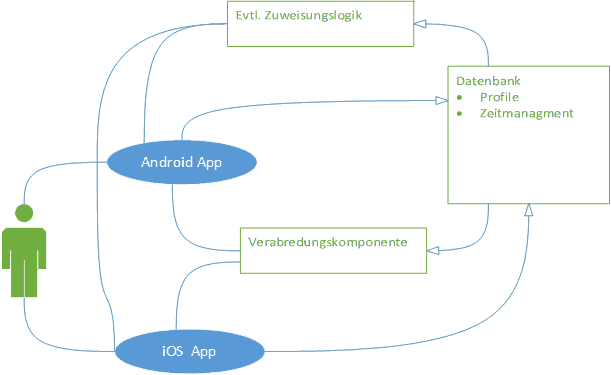
\includegraphics[width=0.75\textwidth]{bilder/useCase.png}
\end{center}

\chapter{Entscheide}

\section{Entscheide zu Vorabklärungen}

\section{Entscheide zu technischen Fragen}

\section{Entscheide zu theokratischen Fragen}
\section{Software}

\subsection{Versionsverwaltung}
Es wird mit GIT gearbeitet (Turtorial\footnote{\url{https://www.kernel.org/pub/software/scm/git/docs/gittutorial.html}})und die Daten liegen auf git-hub{Repository\footnote{\url{https://github.com/priedel/dienstApp}}}. Das Projekt mit \enquote{git clone https://github.com/priedel/dienstApp.git} holen.
 Schreibrechte bei Philipp Riedel (E-Mail\footnote{\href{mailto:riedelp@student.ethz.ch}{riedelp@student.ethz.ch}}) beantragen.

\subsection{Programm Plattform}

Es gibt prinzipiell zwei Möglichkeiten. Pro Betriebssystem wird eine App entwickelt oder es wird mit einer Cross Plattform gearbeitet\cite{appEinf}.


\begin{tabularx}{\textwidth}{lX}
\textbf{individuell}\cite{appEinf}&\\
iOS & mit  Objective-C (oder C/C++)\\
Android & Java \\
\textbf{Cross Plattform}\cite{crossPlat}&\\
    RhoMobile & This is a solution that uses Ruby, especially loved by Ruby on Rails developers. (Free only for noncommercial applications, prices vary)\\
    Appcelerator & This is a solution that allows you to develop native apps with HTML/Javascript (run through a UIWebView on iPhone) . (Free)\\
    PhoneGap & Similar to Appcelerator, I mentioned these two as they seem to have the most vibrant communities, and most extensive support. (Free)\\
    WidgetPad & are good cross platform development tools. Out of these I would rather prefer Phonegap for iOS and Android Development.\\
	Xamarin \footnote{\url{http://www.phoronix.com/scan.php?page=news_item&px=MTUxMzA}}& Xamarin and Microsoft announced a global partnership that enables Microsoft developers to create native mobile Windows, iOS and Android apps with the language they know, C\#, and the tools they love, Visual Studio. This groundbreaking partnership empowers one of the world’s largest developer communities to become the most productive and innovative mobile developers – almost overnight.\\
	\multicolumn{2}{l}{\textbf{WEB mit Schnittstelle zu App oder Native}}\\
	GWT Project \footnote{\url{http://www.gwtproject.org/}} &
	GUI mit GWT zu machen und dann weitere Schnittstellen zu den Spezifischen App zu definieren. Oder GWT Native anzuwenden\\
\end{tabularx}
\centering{{$\vdots$}}

\subsection{Use Case diagramm}
\subsection{Klassendiagramm}

\subsection{Datenbank}



% Nummerierung wieder auf roemisch umschalten
%\newpage
%\pagenumbering{Roman}
%\setcounter{page}{\value{roemisch}}



\chapter{Verzeichnisse}
% Abbildungsverzeichnis
\addcontentsline{toc}{section}{Abbildungsverzeichnis}
\listoffigures

% Tabellenverzeichnis
\addcontentsline{toc}{section}{Tabellenverzeichnis}
\listoftables

% Literaturverzeichnis
\addcontentsline{toc}{section}{Literaturverzeichnis}
%\renewcommand{\refname}{Literaturverzeichnis}
\bibliographystyle{natdin}	%gerplain: [1], geralpha: [Bjar05]
\bibliography{./docFiles/Literatur}


% Appendix, falls vorhanden
\newpage
\numberwithin{table}{chapter}
\begin{appendix}
\section{....}
\end{appendix}


\end{document}
